% GNUPLOT: LaTeX picture with Postscript
\documentclass{minimal}
% Set font size
\makeatletter
\def\@ptsize{7}
\InputIfFileExists{size17.clo}{}{%
   \GenericError{(gnuplot) \space\space\space\@spaces}{%
      Gnuplot Error: File `size17.clo' not found! Could not set font size%
   }{See the gnuplot documentation for explanation.%
   }{For using a font size a file `size<fontsize>.clo' has to exist.
        Falling back ^^Jto default fontsize 10pt.}%
  \def\@ptsize{0}
  \input{size10.clo}%
}%
\makeatother
% Load packages
\usepackage{calc}
\usepackage{graphicx}
\usepackage{color}
\makeatletter
% Select an appropriate default driver (from TeXLive graphics.cfg)
\begingroup
  \chardef\x=0 %
  % check pdfTeX
  \@ifundefined{pdfoutput}{}{%
    \ifcase\pdfoutput
    \else
      \chardef\x=1 %
    \fi
  }%
  % check VTeX
  \@ifundefined{OpMode}{}{%
    \chardef\x=2 %
  }%
\expandafter\endgroup
\ifcase\x
  % default case
  \PassOptionsToPackage{dvips}{geometry}
\or
  % pdfTeX is running in pdf mode
  \PassOptionsToPackage{pdftex}{geometry}
\else
  % VTeX is running
  \PassOptionsToPackage{vtex}{geometry}
\fi
\makeatother
% Set papersize
\usepackage[papersize={514.80bp,501.48bp},text={514.80bp,501.48bp}]{geometry}
% No page numbers and no paragraph indentation
\pagestyle{empty}
\setlength{\parindent}{0bp}%
% Load configuration file
\InputIfFileExists{gnuplot.cfg}{%
  \typeout{Using configuration file gnuplot.cfg}%
}{%
 \typeout{No configuration file gnuplot.cfg found.}%
}%
%
\begin{document}
\begingroup
  \makeatletter
  \providecommand\color[2][]{%
    \GenericError{(gnuplot) \space\space\space\@spaces}{%
      Package color not loaded in conjunction with
      terminal option `colourtext'%
    }{See the gnuplot documentation for explanation.%
    }{Either use 'blacktext' in gnuplot or load the package
      color.sty in LaTeX.}%
    \renewcommand\color[2][]{}%
  }%
  \providecommand\includegraphics[2][]{%
    \GenericError{(gnuplot) \space\space\space\@spaces}{%
      Package graphicx or graphics not loaded%
    }{See the gnuplot documentation for explanation.%
    }{The gnuplot epslatex terminal needs graphicx.sty or graphics.sty.}%
    \renewcommand\includegraphics[2][]{}%
  }%
  \providecommand\rotatebox[2]{#2}%
  \@ifundefined{ifGPcolor}{%
    \newif\ifGPcolor
    \GPcolortrue
  }{}%
  \@ifundefined{ifGPblacktext}{%
    \newif\ifGPblacktext
    \GPblacktextfalse
  }{}%
  % define a \g@addto@macro without @ in the name:
  \let\gplgaddtomacro\g@addto@macro
  % define empty templates for all commands taking text:
  \gdef\gplbacktext{}%
  \gdef\gplfronttext{}%
  \makeatother
  \ifGPblacktext
    % no textcolor at all
    \def\colorrgb#1{}%
    \def\colorgray#1{}%
  \else
    % gray or color?
    \ifGPcolor
      \def\colorrgb#1{\color[rgb]{#1}}%
      \def\colorgray#1{\color[gray]{#1}}%
      \expandafter\def\csname LTw\endcsname{\color{white}}%
      \expandafter\def\csname LTb\endcsname{\color{black}}%
      \expandafter\def\csname LTa\endcsname{\color{black}}%
      \expandafter\def\csname LT0\endcsname{\color[rgb]{1,0,0}}%
      \expandafter\def\csname LT1\endcsname{\color[rgb]{0,1,0}}%
      \expandafter\def\csname LT2\endcsname{\color[rgb]{0,0,1}}%
      \expandafter\def\csname LT3\endcsname{\color[rgb]{1,0,1}}%
      \expandafter\def\csname LT4\endcsname{\color[rgb]{0,1,1}}%
      \expandafter\def\csname LT5\endcsname{\color[rgb]{1,1,0}}%
      \expandafter\def\csname LT6\endcsname{\color[rgb]{0,0,0}}%
      \expandafter\def\csname LT7\endcsname{\color[rgb]{1,0.3,0}}%
      \expandafter\def\csname LT8\endcsname{\color[rgb]{0.5,0.5,0.5}}%
    \else
      % gray
      \def\colorrgb#1{\color{black}}%
      \def\colorgray#1{\color[gray]{#1}}%
      \expandafter\def\csname LTw\endcsname{\color{white}}%
      \expandafter\def\csname LTb\endcsname{\color{black}}%
      \expandafter\def\csname LTa\endcsname{\color{black}}%
      \expandafter\def\csname LT0\endcsname{\color{black}}%
      \expandafter\def\csname LT1\endcsname{\color{black}}%
      \expandafter\def\csname LT2\endcsname{\color{black}}%
      \expandafter\def\csname LT3\endcsname{\color{black}}%
      \expandafter\def\csname LT4\endcsname{\color{black}}%
      \expandafter\def\csname LT5\endcsname{\color{black}}%
      \expandafter\def\csname LT6\endcsname{\color{black}}%
      \expandafter\def\csname LT7\endcsname{\color{black}}%
      \expandafter\def\csname LT8\endcsname{\color{black}}%
    \fi
  \fi
    \setlength{\unitlength}{0.0500bp}%
    \ifx\gptboxheight\undefined%
      \newlength{\gptboxheight}%
      \newlength{\gptboxwidth}%
      \newsavebox{\gptboxtext}%
    \fi%
    \setlength{\fboxrule}{0.5pt}%
    \setlength{\fboxsep}{1pt}%
    \definecolor{tbcol}{rgb}{1,1,1}%
\begin{picture}(10296.00,10029.60)%
    \gplgaddtomacro\gplbacktext{%
      \csname LTb\endcsname%%
      \put(1236,1352){\makebox(0,0)[r]{\strut{}$0$}}%
      \put(1236,2316){\makebox(0,0)[r]{\strut{}$5$}}%
      \put(1236,3281){\makebox(0,0)[r]{\strut{}$10$}}%
      \put(1236,4245){\makebox(0,0)[r]{\strut{}$15$}}%
      \put(1561,819){\makebox(0,0){\strut{}$7$}}%
      \put(2165,819){\makebox(0,0){\strut{}$8$}}%
      \put(2769,819){\makebox(0,0){\strut{}$9$}}%
      \put(3373,819){\makebox(0,0){\strut{}$10$}}%
      \put(3977,819){\makebox(0,0){\strut{}$11$}}%
      \put(4581,819){\makebox(0,0){\strut{}$12$}}%
      \put(5185,819){\makebox(0,0){\strut{}$13$}}%
    }%
    \gplgaddtomacro\gplfronttext{%
      \csname LTb\endcsname%%
      \put(4429,4912){\makebox(0,0)[r]{\strut{}$\tilde{R}_\mathcal{F}$=0, HFB}}%
      \csname LTb\endcsname%%
      \put(4429,4518){\makebox(0,0)[r]{\strut{}$\tilde{R}_\mathcal{F}$=0, BCS}}%
      \csname LTb\endcsname%%
      \put(4429,4124){\makebox(0,0)[r]{\strut{}$\tilde{R}_\mathcal{F}$=1 fm, HFB}}%
      \csname LTb\endcsname%%
      \put(4429,3730){\makebox(0,0)[r]{\strut{}$\tilde{R}_\mathcal{F}$=1 fm, BCS}}%
      \csname LTb\endcsname%%
      \put(403,3174){\rotatebox{-270.00}{\makebox(0,0){\strut{}neutron pairing energy (MeV)}}}%
      \put(3599,309){\makebox(0,0){\strut{}$N_\mathrm{states}^{1/3}$}}%
    }%
    \gplgaddtomacro\gplbacktext{%
      \csname LTb\endcsname%%
      \put(1236,5527){\makebox(0,0)[r]{\strut{}$-20$}}%
      \put(1236,6366){\makebox(0,0)[r]{\strut{}$-15$}}%
      \put(1236,7206){\makebox(0,0)[r]{\strut{}$-10$}}%
      \put(1236,8046){\makebox(0,0)[r]{\strut{}$-5$}}%
      \put(1236,8885){\makebox(0,0)[r]{\strut{}$0$}}%
      \put(1561,4851){\makebox(0,0){\strut{}}}%
      \put(2165,4851){\makebox(0,0){\strut{}}}%
      \put(2769,4851){\makebox(0,0){\strut{}}}%
      \put(3373,4851){\makebox(0,0){\strut{}}}%
      \put(3977,4851){\makebox(0,0){\strut{}}}%
      \put(4581,4851){\makebox(0,0){\strut{}}}%
      \put(5185,4851){\makebox(0,0){\strut{}}}%
    }%
    \gplgaddtomacro\gplfronttext{%
      \csname LTb\endcsname%%
      \put(4429,6687){\makebox(0,0)[r]{\strut{}$\tilde{R}_\mathcal{F}$=0, HFB}}%
      \csname LTb\endcsname%%
      \put(4429,6293){\makebox(0,0)[r]{\strut{}$\tilde{R}_\mathcal{F}$=0, BCS}}%
      \csname LTb\endcsname%%
      \put(4429,5899){\makebox(0,0)[r]{\strut{}$\tilde{R}_\mathcal{F}$=1 fm, HFB}}%
      \csname LTb\endcsname%%
      \put(4429,5505){\makebox(0,0)[r]{\strut{}$\tilde{R}_\mathcal{F}$=1 fm, BCS}}%
      \csname LTb\endcsname%%
      \put(362,7206){\rotatebox{-270.00}{\makebox(0,0){\strut{}charge radius ($10^{-3}$fm)}}}%
      \put(3599,4749){\makebox(0,0){\strut{}}}%
      \put(3599,9731){\makebox(0,0){\strut{}Fy($\Delta r$), $^{120}$Sn, $\varepsilon_\mathrm{cut}$ = 15 MeV}}%
    }%
    \gplgaddtomacro\gplbacktext{%
      \csname LTb\endcsname%%
      \put(5556,1352){\makebox(0,0)[r]{\strut{}}}%
      \put(5556,2316){\makebox(0,0)[r]{\strut{}}}%
      \put(5556,3281){\makebox(0,0)[r]{\strut{}}}%
      \put(5556,4245){\makebox(0,0)[r]{\strut{}}}%
      \put(5881,819){\makebox(0,0){\strut{}$7$}}%
      \put(6485,819){\makebox(0,0){\strut{}$8$}}%
      \put(7089,819){\makebox(0,0){\strut{}$9$}}%
      \put(7693,819){\makebox(0,0){\strut{}$10$}}%
      \put(8296,819){\makebox(0,0){\strut{}$11$}}%
      \put(8900,819){\makebox(0,0){\strut{}$12$}}%
      \put(9504,819){\makebox(0,0){\strut{}$13$}}%
    }%
    \gplgaddtomacro\gplfronttext{%
      \csname LTb\endcsname%%
      \put(8748,4912){\makebox(0,0)[r]{\strut{}$\tilde{R}_\mathcal{F}$=0, HFB}}%
      \csname LTb\endcsname%%
      \put(8748,4518){\makebox(0,0)[r]{\strut{}$\tilde{R}_\mathcal{F}$=0, BCS}}%
      \csname LTb\endcsname%%
      \put(8748,4124){\makebox(0,0)[r]{\strut{}$\tilde{R}_\mathcal{F}$=1 fm, HFB}}%
      \csname LTb\endcsname%%
      \put(8748,3730){\makebox(0,0)[r]{\strut{}$\tilde{R}_\mathcal{F}$=1 fm, BCS}}%
      \csname LTb\endcsname%%
      \put(5709,3174){\rotatebox{-270.00}{\makebox(0,0){\strut{}}}}%
      \put(7919,309){\makebox(0,0){\strut{}$N_\mathrm{states}^{1/3}$}}%
    }%
    \gplgaddtomacro\gplbacktext{%
      \csname LTb\endcsname%%
      \put(5556,5527){\makebox(0,0)[r]{\strut{}}}%
      \put(5556,6366){\makebox(0,0)[r]{\strut{}}}%
      \put(5556,7206){\makebox(0,0)[r]{\strut{}}}%
      \put(5556,8046){\makebox(0,0)[r]{\strut{}}}%
      \put(5556,8885){\makebox(0,0)[r]{\strut{}}}%
      \put(5881,4851){\makebox(0,0){\strut{}}}%
      \put(6485,4851){\makebox(0,0){\strut{}}}%
      \put(7089,4851){\makebox(0,0){\strut{}}}%
      \put(7693,4851){\makebox(0,0){\strut{}}}%
      \put(8296,4851){\makebox(0,0){\strut{}}}%
      \put(8900,4851){\makebox(0,0){\strut{}}}%
      \put(9504,4851){\makebox(0,0){\strut{}}}%
    }%
    \gplgaddtomacro\gplfronttext{%
      \csname LTb\endcsname%%
      \put(8748,6687){\makebox(0,0)[r]{\strut{}$\tilde{R}_\mathcal{F}$=0, HFB}}%
      \csname LTb\endcsname%%
      \put(8748,6293){\makebox(0,0)[r]{\strut{}$\tilde{R}_\mathcal{F}$=0, BCS}}%
      \csname LTb\endcsname%%
      \put(8748,5899){\makebox(0,0)[r]{\strut{}$\tilde{R}_\mathcal{F}$=1 fm, HFB}}%
      \csname LTb\endcsname%%
      \put(8748,5505){\makebox(0,0)[r]{\strut{}$\tilde{R}_\mathcal{F}$=1 fm, BCS}}%
      \csname LTb\endcsname%%
      \put(5709,7206){\rotatebox{-270.00}{\makebox(0,0){\strut{}}}}%
      \put(7919,4749){\makebox(0,0){\strut{}}}%
      \put(7919,9731){\makebox(0,0){\strut{}Fy($\Delta r$), $^{120}$Sn, $\varepsilon_\mathrm{cut}$ = 45 MeV}}%
    }%
    \gplbacktext
    \put(0,0){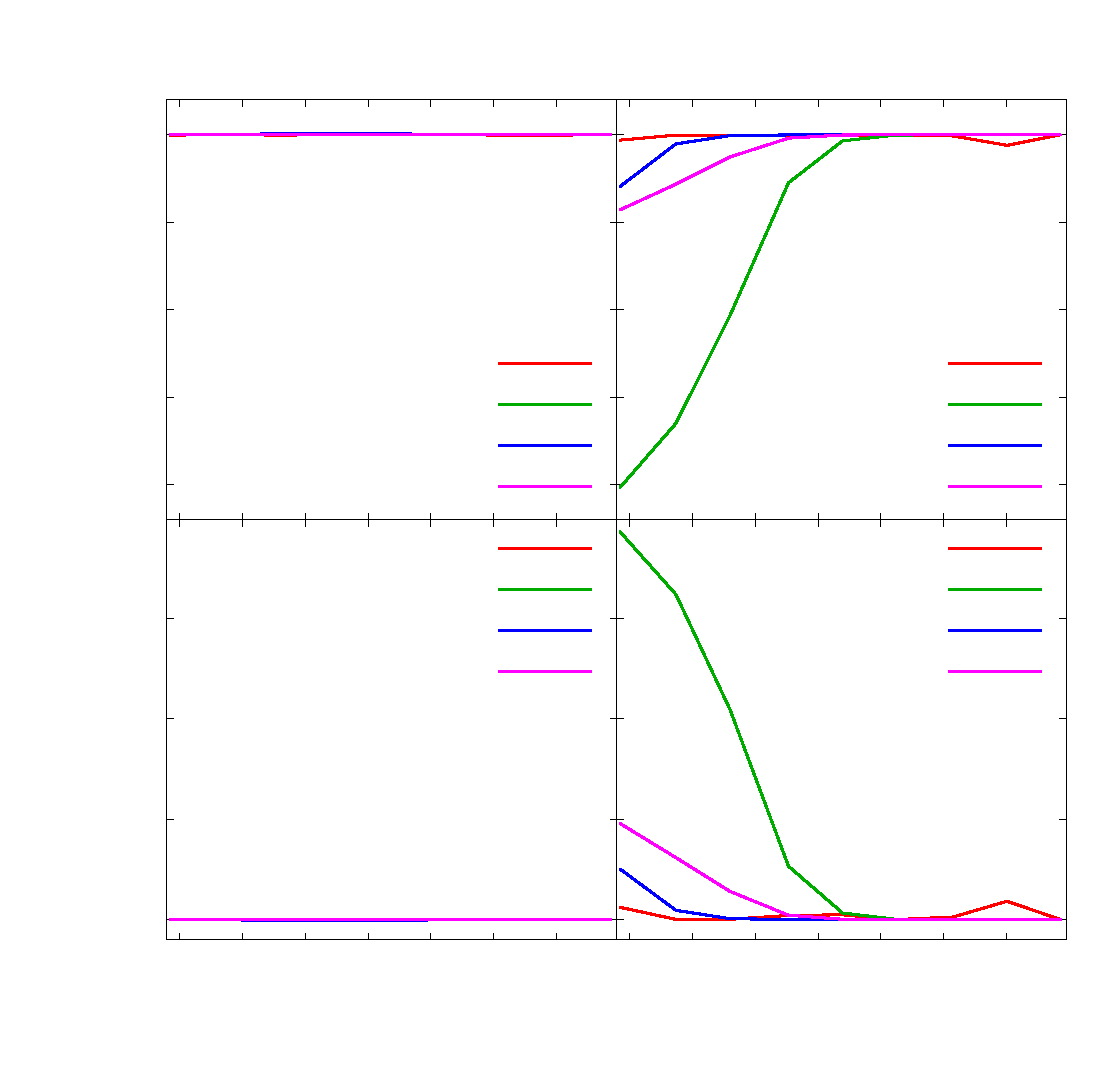
\includegraphics[width={514.80bp},height={501.48bp}]{Sn120-varydeocc_cut15_2-inc}}%
    \gplfronttext
  \end{picture}%
\endgroup
\end{document}
